%=================================================%
%-->    Lab: Digital Basics, Counter and Timer <--%
%--> Author: Charles Edward Pax                <--%
%-->   Date: 2006.03.21                        <--%
%=================================================%
%
\documentclass[11pt,onecolumn,letter]{article}
\usepackage{color,graphics}

\begin{document}
\title{Digital Basics, Counter and Timer}
\date{\today}
\author{Charles Edward Pax}
\maketitle

%=====================%
%--> Sec: Abstract <--%
%=====================%
\abstract{A logic chip, flip-flop, timer, and counter are each used in various circuits and their behiviour observed.}

%=========================%
%--> Sec: Introduction <--%
%=========================%
\section{Introduction}\label{sec:Introduction}
NAND logic gates can be used to construct any other type of logic gate. In this report the NOT, AND, and OR gates are constructed using the 74LS00 IC.

The 555 timer circuit can be used to drive a flipflop circuit. Several flipflop circuits can be cascaded together to form a $n$-bit binary counter with the 555 acting as the driver. Such a configuration can also be referred to as a {\em divide-by-$2^n$} circuit because each flipflop in the cascade divides the frequency of the flipflop before it by two.

A 7448 IC can be used to conver the signal from several flipflop circuits into a form more readily usable in a 7-segment digital display.

%============================%
%--> Sec: Data & Analysis <--%
%============================%
\section{Data \& Analysis}\label{sec:DataAnalysis}
%
% Subsection: Quad NAND 74LS00
%
\subsection{Quad NAND 74LS00}\label{subsec:QuadNAND}
The 74LS00 in Figure \ref{fig:74LS00} houses four dual input NAND logic gates. Each logic gate was first checked to ensure proper function by placing the low-voltage leg of a LED to the output of each logic gate. This was done due to the IC's inability to supply enough current to active the LED. Doing this meant that the lighting of the LED meant low voltage or FALSE while the absance of light meant high voltage or TRUE.
%
% Figure: 74LS00
%
\begin{figure}
\center

\includegraphics{74LS00.eps}
\caption{74LS00 dual guad NAND IC.}\label{fig:74LS00}
\end{figure}

A NOT gate, shown in Figure \ref{fig:NOT}, AND gate, shown in Figure \ref{fig:AND}, and an OR gate, shown in Figure \ref{fig:OR} were each constructed using NAND gates. The output was shown to the instructor. The truth tables for the NOT, AND, and OR gates are respectivly shown in Table \ref{tab:NOT}, Table \ref{tab:AND}, and Table \ref{tab:OR}.
%
% Figure: NOT
%
\begin{figure}
\center
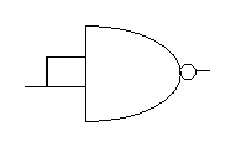
\includegraphics{NOT.eps}
\caption{NOT gate composed of a NAND gate.}\label{fig:NOT}
\end{figure}
%
% Table: NOT Gate
%
\begin{table}
\center
\begin{tabular}{ccc}
	& NOT Gate	& \\
\hline
Pin 1	& Pin 2	& Pin 6 \\
\hline
0	& 0	& 1 \\
1	& 1	& 0 \\
\end{tabular}
\caption{NOT gate. Pin numbers correspond to the pins on the 74LS00 TTL IC. Pins 1 and 2 are inputs, pin 3 is the output.}\label{tab:NOT}
\end{table}
%
% Figure: AND
%
\begin{figure}
\center
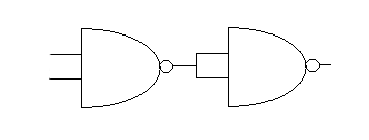
\includegraphics{AND.eps}
\caption{AND gate composed of NAND gates.}\label{fig:AND}
\end{figure}
%
% Table: AND Gate
%
\begin{table}
\center
\begin{tabular}{ccc}
	& AND Gate	& \\
\hline
Pin 1	& Pin 2	& Pin 6 \\
\hline
0	& 0	& 0 \\
0	& 1	& 0 \\
1	& 0	& 0 \\
1	& 1	& 1 \\
\end{tabular}
\caption{AND gate. Pin numbers correspond to the pins on the 74LS00 TTL IC. Pins 1 and 2 are the inputs whose output on pin 3 acts as the input of pins 4 and 5, where pin 6 is the final output.}\label{tab:AND}
\end{table}
%
% Figure: OR
%
\begin{figure}
\center
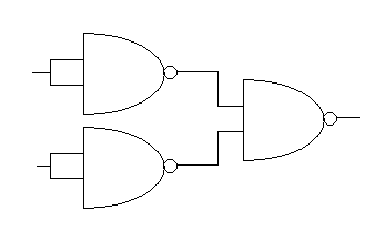
\includegraphics{OR.eps}
\caption{OR gate composed of NAND gates.}\label{fig:OR}
\end{figure}
%
% Table: OR Gate
%
\begin{table}
\center
\begin{tabular}{ccc}
	& OR Gate	& \\
\hline
Pin 1	& Pin 5	& Pin 8 \\
\hline
0	& 0	& 0 \\
0	& 1	& 1 \\
1	& 0	& 1 \\
1	& 1	& 1 \\
\end{tabular}
\caption{OR gate. Pin numbers correspond to the pins on the 74LS00 TTL IC. Pins 1 and 5 are the inputs, pin 8 is output.}\label{tab:OR}
\end{table}

%
% Subsection: 555 Timer
%
\subsection{555 Timer}\label{subsec:555Timer}
The 555 timing circuit shown in Figure \ref{fig:555Timer} was constructed using the following values: $C = 1000$ pF, $R_a = 330$ k$\Omega$, and $R_b = 470$ k$\Omega$. The resultant wave form is shown in Figure \ref{fig:555Square}. The amplitude is 10.5 mV. As can be seen from the Figure \ref{fig:555Square}, the charging process occures asymtopticly towards its maximum value and the discharging exponentially decays to its minimum value. The charging time is is given by equation \ref{eq:555Charging}
%
%
%
\begin{figure}
\center
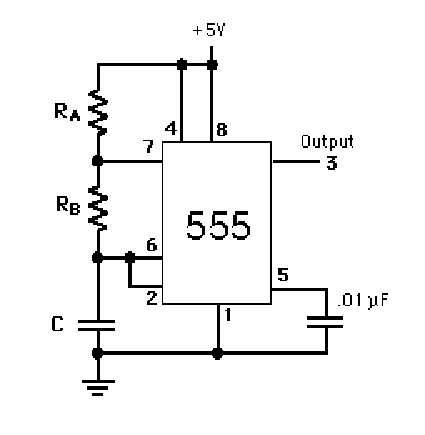
\includegraphics{555Timer.eps}
\caption{555 timer circuit.}\label{fig:555Timer}
\end{figure}
%
% Equation: 555 Charging
%
\begin{equation}\label{eq:555Charging}
t_{charging} = 0.695 (R_a + R_b) C
\end{equation}
and for $C = 1000$ pF, $R_a = 330$ k$\Omega$, and $R_b = 470$ k$\Omega$ is calculated as
\begin{displaymath}
t_{charging} = 0.695 (330000 + 470000) 1 \cdot 10^{-9}
\end{displaymath}
\begin{displaymath}
t_{charging} = 5.56 \cdot 10^{-4}\ \mathrm{s}
\end{displaymath}
The measured value of 3.3 $\cdot$ 0.2 ms $= 6.6 \cdot 10^{-4}$ s is withing 16\% of the calculated $5.56 \cdot 10^{-4}\ \mathrm{s}$.

The discharging time is given by equation \ref{eq:Discharging}
%
% Equation: 555 Discharging
%
\begin{equation}\label{eq:Discharging}
t_{discharging} = 0.695 R_a C
\end{equation}
and for $C = 1000$ pF, and $R_b = 470$ k$\Omega$ is calculated as
\begin{displaymath}
t_{discharging} = 0.695 \cdot 470000 \cdot 1 \cdot 10^{-9}
\end{displaymath}
\begin{displaymath}
t_{discharging} = 3.27 \cdot 10^{-4}\ \mathrm{s}
\end{displaymath}
The measured value of $2 \cdot 0.2$ ms $= 4.0 \cdot 10^{-4}$ s is within 19\% of the calculated $3.27 \cdot 10^{-4}\ \mathrm{s}$.
%
% Figure: 555 Square
%
\begin{figure}
\center
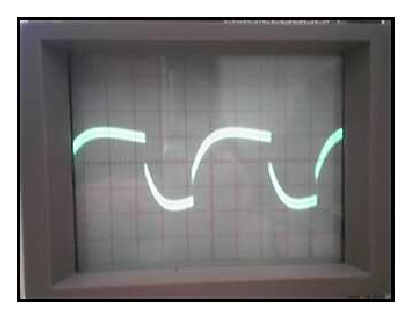
\includegraphics{square.eps}
\caption{555 timer output. Sweep time = 0.2 ms, voltage scale = 5 mV, amplitude is 10.5 mV.}\label{fig:555Square}
\end{figure}

Figure \ref{fig:555Triangle} shows the trigger input of the 555 timer circuit.
%
% Figure: 555 Triangle
%
\begin{figure}
\center
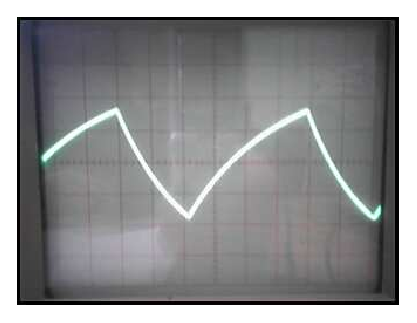
\includegraphics{triangle.eps}
\caption{555 timer trigger input. Sweep time = 0.2 ms, voltage scale = 0.5 V, amplitude = 0.875 V.}\label{fig:555Triangle}
\end{figure}
These results agree with expectations in that the off time is less than the on time and the wave forms are accurate to calculations.

Capacitor $C$ was changed to 1 $\mu$F and a LED was put on pin 3. The frequency of the blinking LED was measured over ten cycles twice to give (8.01 + 7.94)/20 = 0.8 Hz.

%
% Subsection: 7474 D-type Flipflop
%
\subsection{7474 D-type Flipflop}\label{subsec:Flipflop}
The output of the 555 timer circuit was connected to the input of a 7474 D-type flipflop logic unit as shown in Figure \ref{fig:Flipflop}. This circuit divides the frequency of the timer by two because the state of the fliflop IC changes only when the timer returns to a low voltage from a high voltage as shown in figure \ref{flipflopChart}.
%
% Figure: Flipflop
%
\begin{figure}
\center
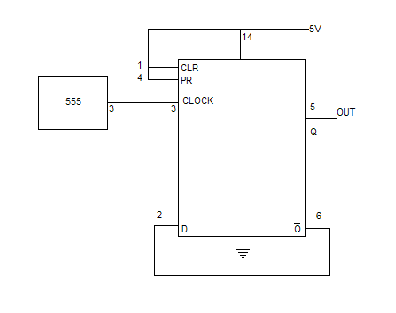
\includegraphics{flipflop.eps}
\caption{D-type flipflop and 555 timer circuit diagram.}\label{fig:Flipflop}
\end{figure}
%
% Figure: Flipflop Chart
%
\begin{figure}
\center
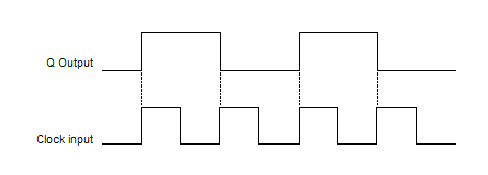
\includegraphics{flipflopChart.eps}
\caption{Oscillation chart for flipflop and 555 timer.}\label{flipflopChart}
\end{figure}

%
% Subsection: Binary Counter
%
\subsection{Binary Counter}\label{subsec:BinaryCounter}
Chaining together several flipflops one can construct divide-by-$2^n$ circuits. Four flipflops in two 7474 ICs were linked together (see Figure \ref{fig:BinaryCounter}) to give a cascading counting effect (see Figure \ref{fig:oscillationChart}; a divide-by-16 circuit or a 4 bit digital counter. It was observed and demonstrated to the instructor that each flipflop LED blinked at half the rate of the one before it with each LED starting as illuminated to indicate a low voltage or FALSE.
%
% Figure: Binary Counter
%
\begin{figure}
\center
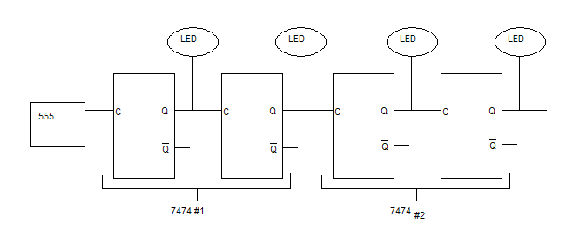
\includegraphics{BinaryCounter.eps}
\caption{}\label{fig:BinaryCounter}
\end{figure}
%
% Figure: Oscillation Chart
%
\begin{figure}
\center
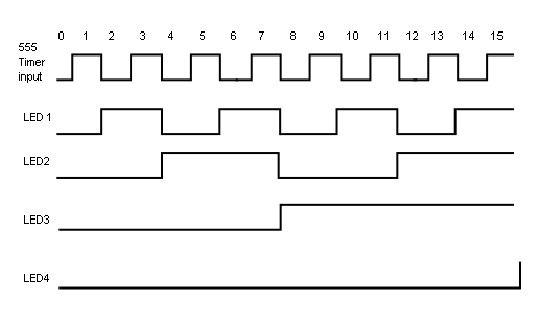
\includegraphics{oscillationChart.eps}
\caption{Oscillation chart.}\label{fig:oscillationChart}
\end{figure}

%
% Subsection: Counter Display
%
\subsection{Counter Display}\label{subsec:CounterDisplay}
A 7-segment LED display can be used to show the state of the 4 bit digital counter for numbers 0 through 9. A 7448 BCD decoder chip is used to translate the outputs of the four flipflops into a signal usable with a 7-segment LED display. Figure \ref{fig:display} shows the progression of the 7-segment digital display. The display shows nonnumbers for the values from 10 to 15. The pins of the 7448 are connected to the $\bar{Q}$ of each flipflop rather than the $Q$ so that the lighting of a LED indicated TRUE. This gives the proper display that we are used to where the number is represented by light. As the cycle progresses the counter begins at 0 and counts up to 9.
%
% Figure: Display
%
\begin{figure}
\center

\includegraphics{display.eps}
\caption{Digital display cycle.}\label{fig:display}
\end{figure}

%=====================================%
%--> Sec: Discussion & Conclusions <--%
%=====================================%
\section{Discussion \& Conclusions}\label{sec:DiscussionConclusions}
Using simple ICs and anaglog components one can construct a fairly complex circuit that does a highly useful task. Digital counters have become common in today's world and are easy to take for granted. By performaing this lab it can be seen how a clock or other counter can be made using simple parts.

\end{document}
